\chapter{Visual Effects}
\thispagestyle{fancy}
\section{Was sind Visual Effects?}
Bevor der Term \textit{Visual Effects} definiert wird, soll klargestellt werden, dass das Wort \textit{Film} im weiteren Verlauf dieser Arbeit alle Bewegtbildproduktionen einschließt und sich nicht ausschließlich auf narrativen Film bezieht.\\

Eine passende Definition für Visual Effects (VFX) gibt die \textit{Visual Effects Society}. Diese bezeichnet Visual Effects als Bilder, die für einen Film erschaffen, geändert oder erweitert wurden und solche, die in dieser Art nicht vor Ort am Filmset hätten aufgenommen werden können \parencite[S. 2]{okun2020ves}. Eine weitere Beschreibung dieses Begriffes lässt sich aus dem Buch \textit{visual effects for film and
television} entnehmen: 
\begin{quote}
\glqq However, ironically, so called ‘visual’ effects would not necessarily be visible
to the casual observer standing nearby. They can be defined as where the components of the photographic process are utilized or modified so as to alter in
some non-standard way the passage of light creating the image. Thus, you might
replace the background with a photographic element such as a photo-blow-up,
filter the light being used on the set in some specialized way, filter or mask the
lens, run the camera at an abnormal speed or interfere with the processing
between image capture and presentation. All of these might be components in a
process to modify the image, but with the final result being unobservable on the
actual set.\grqq{} \parencite[S. 9]{mitchell2013visual}\end{quote}

Die Definitionen unterscheiden sich darin, dass Okun et al. den Prozess der Visual Effects als einen Vorgang ansehen, der nach dem Dreh passiert, während Mitchell beispielsweise auch Modifizierungen der Kameralinse während des Drehs als Visual Effect bezeichnet. Bei beiden Definitionen fällt auf, dass Filmmaterial, welches im Nachhinein mit speziellen Effekten versehen wurde, als Visual Effects zu beschreiben ist. Dieses Hauptmerkmal aus beiden Definitionen ist auch die Grundlage für die Definition in dieser Arbeit. \\

Visual Effects entstehen nun also nach dem Dreh und die englische Bezeichnung der \textit{Postproduction} ist hierbei sehr treffend. 
Mittlerweile findet die Postproduction meist rein digital statt und es wurden eine Reihe an neuen Filmgewerken entwickelt, welche diese Nachbearbeitung abwickeln. \citet[]{fis-eireann-2019} erklärt, dass es mehrere Gewerke innerhalb einer VFX-Produktion gebe. Diese können grob in drei Parteien aufteilt werden: die \textit{Production}, welche sich um die Organisation der zu bearbeitenden, Filmausschnitte, den sogenannten \textit{Shots} kümmert, \textit{Artists}, welche mit verschiedensten Programmen arbeiten und sich um die kreative Gestaltung der Shots kümmern und zuletzt die \textit{Technical Directors}. Sie lösen komplexe Probleme und Aufgaben innerhalb der Programme oder arbeiten mittels Softwareentwicklung an den Programmen selbst, um einen reibungslosen Ablauf der Produktion im Bezug auf die eingesetzten Programme zu garantieren. Natürlich sind das nur grobe Beschreibungen der Aufgaben innerhalb der Parteien. In der Postproduction fließen also verschiedene Arbeitsschritte zusammen, die einen Film auf eine komplett andere visuelle Ebene heben können.


\section{Was ist CGI?}
Der Term \textit{Computer Generated Imagery} (CGI) beschreibt Bilder, die nicht mit einer Kamera aufgenommen wurden, sondern rein digital entstanden sind \parencite[]{jacobs-2022}. Computer Generated Imagery lassen sich in eine Unterkategorie zu Visual Effects einordnen, können aber auch für sich allein stehen, wenn der Begriff in anderen Bereichen außerhalb des Films verwendet wird. Solche Bilder finden sich beispielsweise auch in Computerspielen, im Fernsehen und anderen Medien, um Werbung oder andere Inhalte zu gestalten. Dabei muss es sich aber nicht um das komplette Bild handeln, denn es ist ebenso ausreichend nur kleine Teile oder Objekte virtuell umzusetzen. \citet[]{feldman-2019} erklärt, dass die Drachen der Fernsehserie \textit{Game Of Thrones} virtuell am Computer erstellt und animiert wurden, damit sie im Nachhinein in einen Shot eingebaut werden konnten. Er führt fort, dass die Darstellerin, welche am Filmset mit dem Drachen agieren sollte, anstatt mit dem Drachen, mit einer dem Drachen ähnelnden Konstruktion agierte und diese Konstruktion durch den virtuellen Drachen ersetzt wurde.\\

Digital kreierte Bilder sind essenziell für die Visual Effects Branche, denn sie ermöglichen eine Komposition von Realfilmaufnahmen mit digitalen Elementen. CGI ist aber nicht nur auf eine Komposition aus verschiedenen Bildquellen beschränkt, denn es werden auch häufig ganze Filme ohne jeglichen Realfilmanteil erstellt. Nach \citet[]{garcia-no-date} werden sie als sogenannte \textit{Full CG} Filme bezeichnet. Dafür müssen alle Elemente des Films in 3D nachgebildet werden und es entsteht eine lange Kette an Arbeitsschritten bis zum finalen Produkt. Gegenstände müssen modelliert, Charaktere erschaffen sowie animiert werden. Landschaften werden aus verschiedensten Elementen und Texturen komponiert und alle diese Bausteine fließen am Ende zusammen, um die uns bekannte oder eine alternative Realität zu erschaffen. 

\section{Definition: Simulation}
Ein wichtiger Teil von Visual Effects ist unter anderem, dass virtuelle Objekte in einer Szene mit sich, aber auch den realen Elementen im Film interagieren sollen und sich dabei physikalisch korrekt verhalten. Beispielsweise soll ein 3D-Charakter in Flammen aufgehen oder ein nicht reales Piratenschiff soll simulierte Wellen auf dem Meer hinter sich ziehen. Eine erste Erläuterung zur Funktionsweise von Simulationen bietet ihre Definition. Nach \citet[]{Discrete-Event} sei eine Simulation die Imitation einer Funktion eines Real-Prozesses oder eines Systems über Zeit. Die Autoren führen fort, dass eine Simulation die Generation einer künstlich geschaffenen Historie bedarf, um Schlussfolgerungen auf das System in der echten Welt ziehen zu können.\\

In Abbildung \ref{fig:moana} ist ein der Vergleich einer Feuer- und Rauchsimulation zu sehen, während ihrer Konzeption und im fertigen Film. Um solche Bilder zu realisieren, kommen verschiedenste Arten von Simulationen zum Einsatz, die mithilfe spezieller Programme und Verfahren am Computer errechnet werden. \\

\begin{figure}[ht]
    \centering
    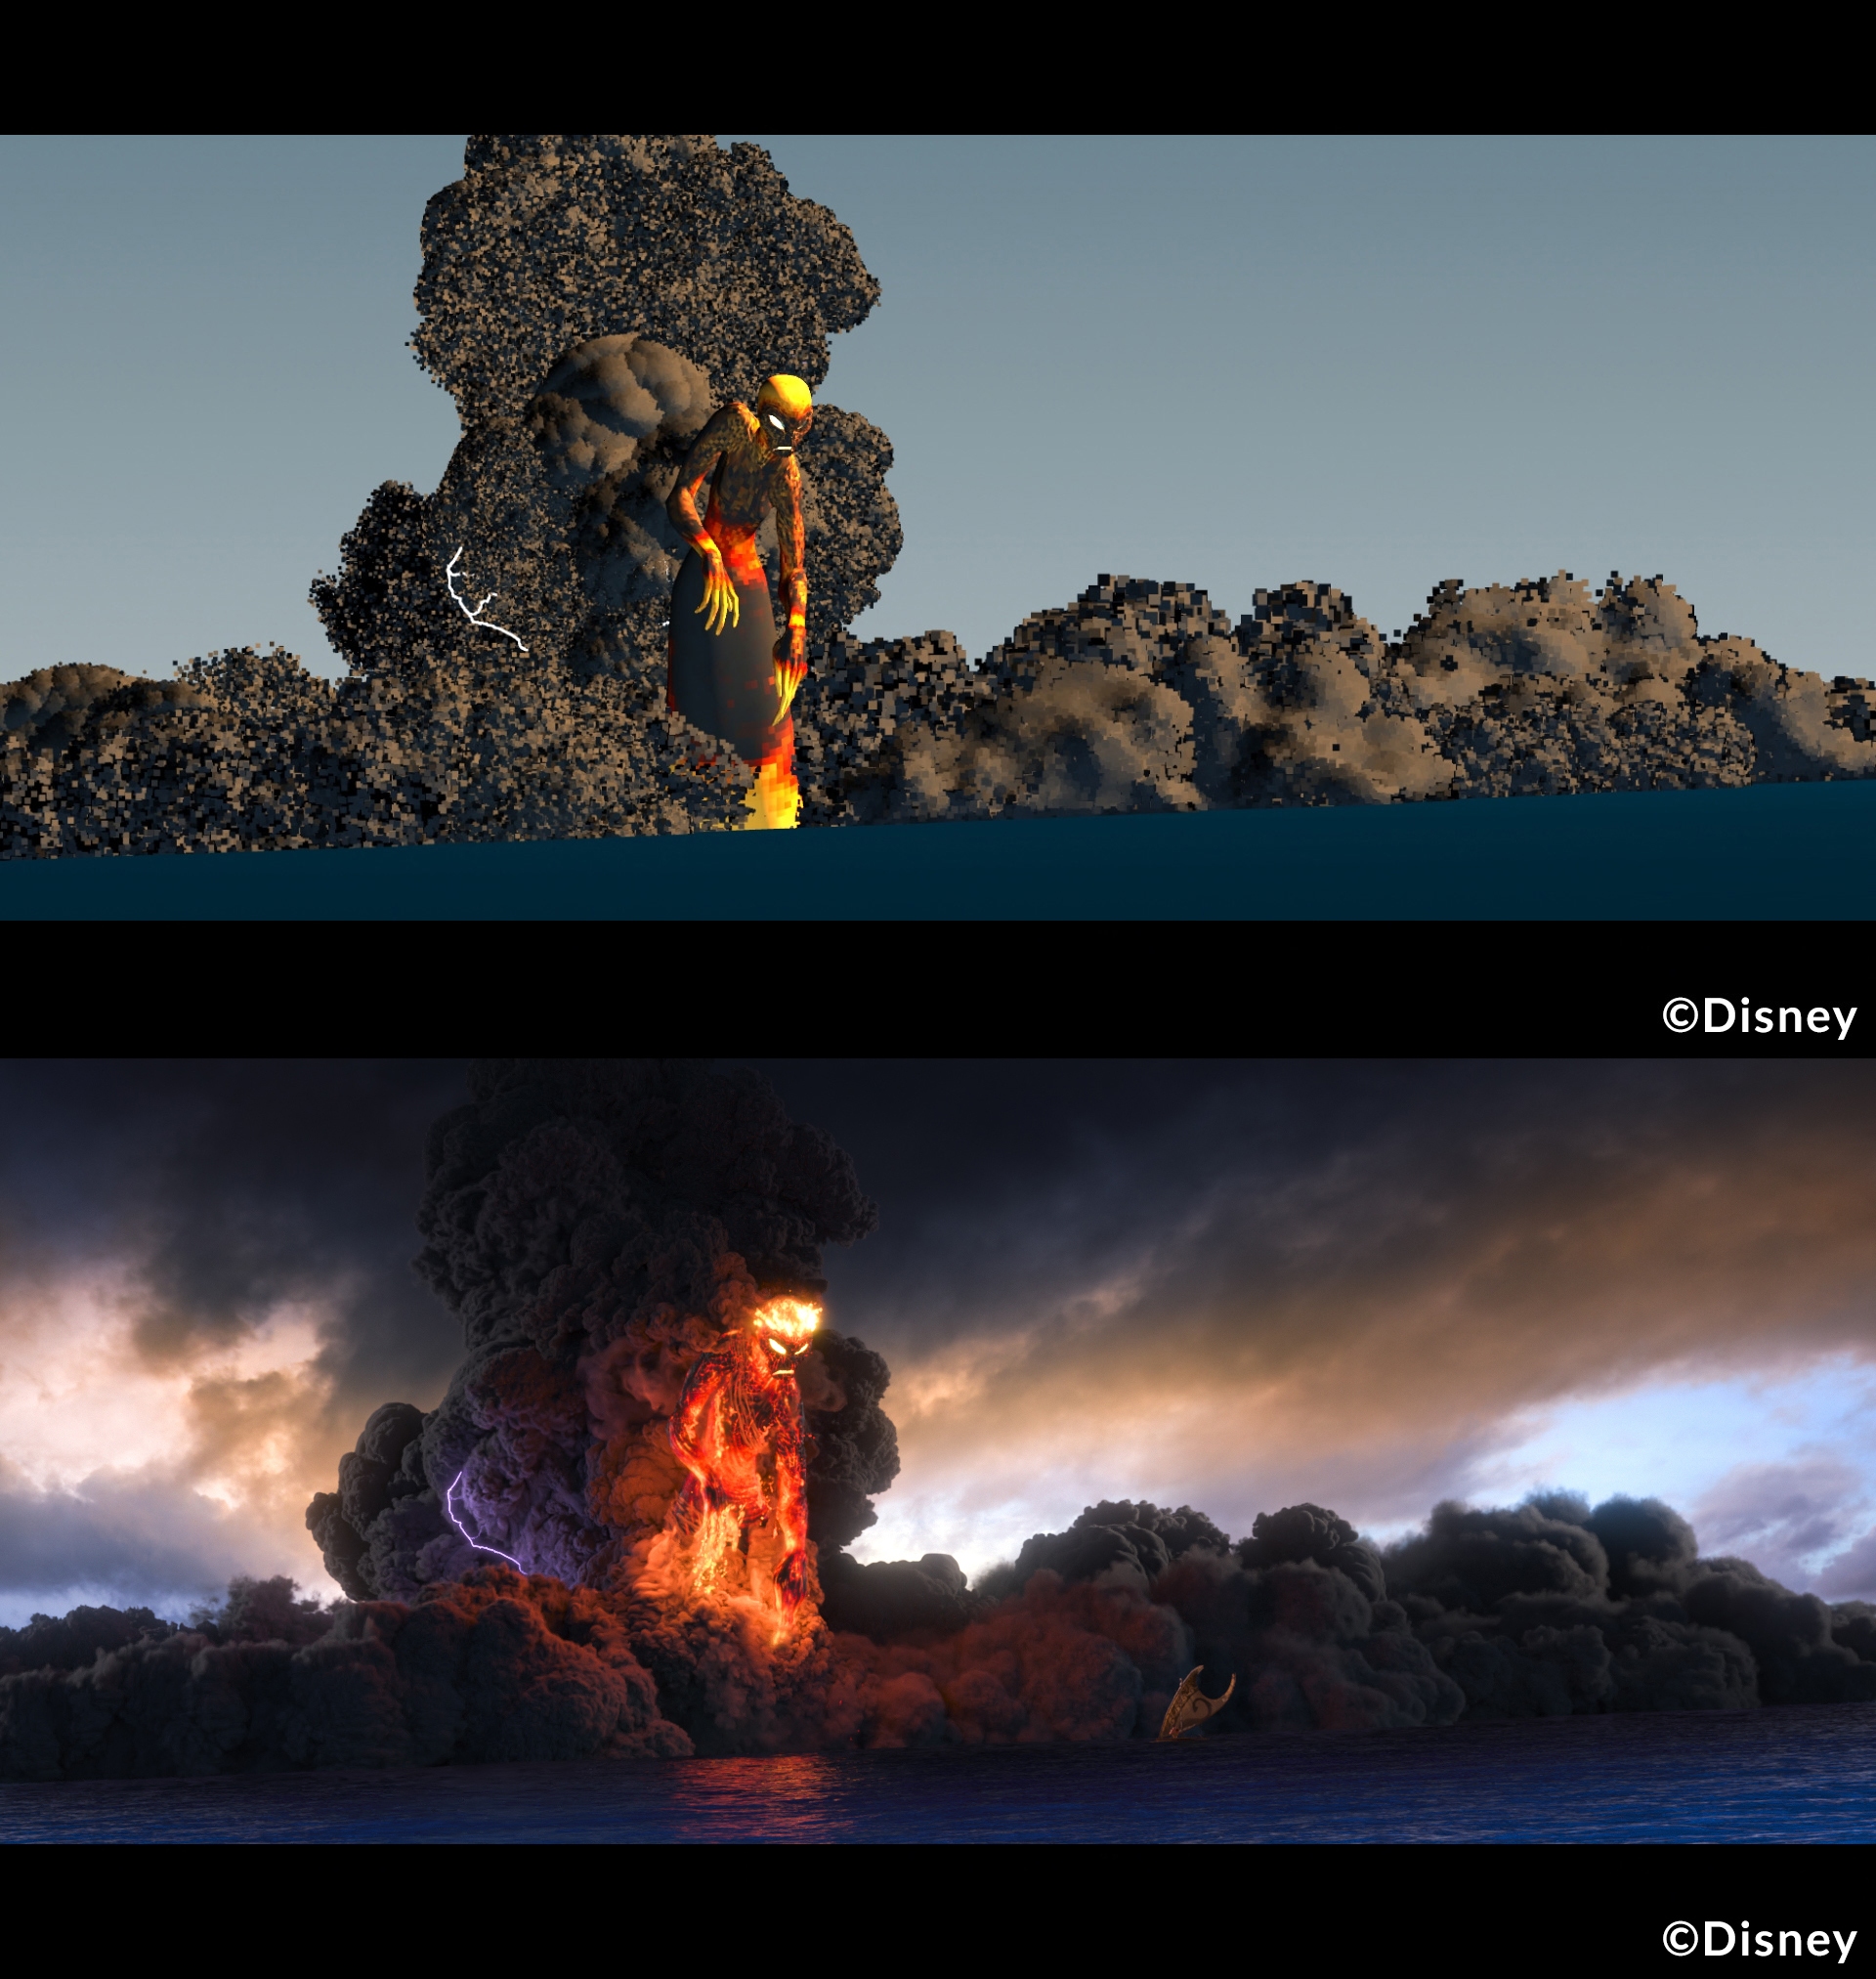
\includegraphics[width=12cm]{bilder/vaiana.jpg}
    \caption{Vorher-Nachher-Vergleich der Simulationen eines Shots aus dem Film \glqq Moana\grqq{} (2016).}
    \source{\citet[]{side-effects-software-2017}}
    \label{fig:moana}
\end{figure}



Wie lässt sich diese Definition jetzt in die Visual Effects Welt übertragen? Zwei Elemente sind hierfür wichtig: die Zeit und die auf ihr basierende Historie. Als Beispiel für den realen Prozess soll eine Explosion in 3D repliziert werden. Zu Beginn sei ein Emitter an einer bestimmten Position im 3D-Raum, der Schritt für Schritt Rauch und Flammen in den leeren Raum emittiert, über eine vom Nutzer bestimmte Zeit hinweg. Die Schritte sind in diesem Fall die einzelnen Bilder eines Films, auch \textit{Frames} genannt. Im ersten Frame ist die Explosion gering und hat viel Energie, die dafür sorgt, dass sich das Feuer und der Rauch ausbreiten können. Im zweiten Frame breitet sich die Explosion stark aus, während ihr Energielevel sinkt. Die Simulation entwickelt sich über mehrere Sekunden, bis ihre Energie aufgebraucht ist und die Flammen und der Rauch langsam verschwinden. Jeder Frame in einer Simulation muss auf dem Vorherigen aufbauen, damit der physikalisch korrekte Ablauf gewährt ist. Das bedeutet, dass dieses System von Frame zu Frame deterministischen Algorithmen unterliegt, also dass für dieselbe Eingabe stets dasselbe Ergebnis erzeugt wird. So lässt sich mit den vorhandenen Daten zur Energie immer vorhersagen, wie der nächste Frame aussehen wird. Bei einer 100 Frames langen Simulation ist es jedoch nicht möglich, erst den letzten Frame zu simulieren, denn es ist nicht bekannt, wie sich die Simulation in den 99 vorherigen Frames entwickelt hat. So bedarf es also einer Historie an Frames, die aufeinander aufbauen, aus der wir schlussfolgern können, wie sie sich für den 101 Frame entwickeln würde, wenn alle 100 Frames davor bereits simuliert wurden.\\

Solche Simulationen tragen erheblich zum Realismus eines Filmes bei, sind aber sehr aufwendig in ihrer Herstellung. Für die Visual Effects der Amazon Serie \textit{Star Treck Picard  (2020)}, unter anderem erstellt von Mackevison, wurde zum Beispiel ein auf einer Wassersimulation basierender Wurmloch-Effekt über mehrere Tage hinweg simuliert, um diesen später zu rendern und in einen Shot zu integrieren. Die Berechnung eines Frames dauerte im Schnitt acht Minuten und benötige 25 Gigabyte Speicherplatz. Für die insgesamt 750 Frames ergibt sich eine Simulationszeit von circa vier Tagen und ein Speicherplatzverbrauch von 18 Terabyte. Meistens ist eine Version einer Simulation nicht genug, sondern es werden einige Iterationen benötigt, um Verbesserungen und Kundenwünsche zu integrieren. So zeigt sich, dass es für ein Unternehmen im VFX-Bereich äußerst wertvoll ist, diese Prozesse zu beschleunigen und datensparsamer zu gestalten. Ein schnelleres Iterieren von Simulationen ermöglicht es dem Artist mehrere solcher Aufgaben in derselben Zeit zu bewältigen und Simulationen, die weniger Speicherplatz verbrauchen, würden eine große Kostenersparnis darstellen.

\section{Arten von Simulationen im VFX-Bereich}
Dieser Abschnitt soll einen Überblick über die verschiedenen Arten von Simulationen im VFX Bereich geben. Zuerst folgt ein Exkurs in den Aufbau und die Struktur eines 3D-Modells, denn die verschiedenen Simulationsarten gehen teilweise unterschiedlich mit dieser Struktur um. Die Erläuterungen beziehen sich stets auf die 3D-Simulations-Software \textit{Houdini} des Herstellers \textit{SideFX} \parencite[]{houdini}. Die Wahl Houdini als Programm für das Erzeugen der Simulationen zu nutzen, basierte auf dessen häufigen Einsatz in VFX-Unternehmen. Laut \citet[]{kim-2022} hat sich Houdini bei einer breiten Masse an Film- und VFX-Unternehmen etabliert. Auch Mackevision nutzt Houdini, um eine Vielzahl an Filmeffekten zu simulieren.

\begin{figure}[ht]
    \centering
    \includegraphics[width=8cm]{bilder/wireframe.jpg}
    \caption{Wireframe Ansicht eines 3D-Modells.}
    \source{Bild: Philipp Benner, Modell: Rico Cilliers}
    \label{fig:wire}
\end{figure}

\citet[]{menace-2021} nach, bestünden 3D-Modelle grundlegend aus Punkten, den sogenannten \textit{Vertices}, welche an bestimmten Koordinaten im dreidimensionalen Raum platziert seien. Um nun die Illusion eines geschlossenen Körpers zu erzeugen, würden drei oder vier Punkte miteinander verbunden, um eine Fläche zu schaffen. Drei Punkte würden ein Dreieck oder \textit{Triangle} und vier Punkten ein \textit{Quad} (eng. Quadrilateral für Viereck) erzeugen. Abbildung \ref{fig:wire} zeigt im mittleren Bildausschnitt das Modell als \textit{Mesh, Wireframe oder auch Drahtmodell} bestehend aus Quads. Letztlich werden die Punkte des Modells und die Verbindungslinien oder \textit{Edges} pro Punkt zu seinen Nachbarn gespeichert. Dies sind die grundlegenden Informationen, mit denen in den folgenden Simulationen gearbeitet wird.

\subsection{Rigid Body Simulations} 
Zu Deutsch \textit{Starrkörpersimulationen}. Sie werden verwendet, um Objekte zu bewegen oder sie mit anderen Objekten kollidieren zu lassen. Wie der Name schon andeutet, sind diese Objekte starr und nicht verformbar. Als Beispiel dient eine Bowlingkugel und Bowling-Pins auf einer Bahn. Die Kugel erhält eine initiale Geschwindigkeit in Richtung der Pins, rollt die Bahn entlang und kollidiert mit ihnen. Die Verbindungslinien der Punkte im Mesh behalten dabei stets ihre Länge und Rotation zueinander. Sollen die Objekte verformbar sein, so kommen \textit{Soft Body Simulations} zum Einsatz. Dabei lässt sich die Länge und Rotation der Edges zu den anderen Punkten verändern. So können sich Teile des Modells zusammenziehen, strecken und falten \parencite[]{baraff-2001}.

\subsection{Particle Simulations} 
Sie sind die simpelste Form der Simulationen. Dabei werden nur einzelne Punkte, ohne Edges oder Flächen simuliert. Durch Kräfte wie Wind, Gravitation oder Magnetismus wird ihre Bewegung im Raum über Zeit berechnet. Erhalten die Partikel noch ein Attribut wie eine Lebensspanne, lassen sie sich nach einer gewissen Zeit aus der Simulation entfernen oder langsam ausblenden. Meist haben die Partikel keine Größe während der Simulation und sind theoretisch gesehen unendlich klein \parencite[]{reeves}. Später, während des Renderings, also dem Errechnen des fertigen Bildes aus den 3D-Daten, wird an die Position eines Punktes eine winzige Kugel mit einem gewissen Radius gesetzt, um das Partikel im Bild sichtbar zu machen \parencite[]{sidefxparicle}. Viele magische Filmeffekte nutzen diese Art der Simulation, dann aber mit Millionen von Partikeln, um den Eindruck einer festen Materie zu erwecken.

\subsection{Pyro Simulations} 
Solche Simulationen nutzen eine gänzlich andere Struktur, um Flammen und Rauch zu simulieren. Dabei spielen Punkte und Edges keine Rolle mehr, sondern nutzen sogenannte \textit{Voxel}. Dieser Begriff leitet sich von \textit{Volume Elements} \parencite[S. 549]{FoleyDamEtAl90} ab und beschreibt einen Würfel, der ein Teil eines dreidimensionalen Rasters ist. Abbildung \ref{voxel} zeigt ein Pixelbild der Zahl 5. Anhand der Helligkeitswerte der Pixel ist erkennbar, dass einige Pixel den Wert eins haben, was bedeutet, dass sie zu 100\% weiß sind. Andere Pixel hingegen sind etwas dunkler und haben geringere Helligkeitswerte. Dieses Prinzip lässt sich von einem zweidimensionalen in ein dreidimensionales Raster übertragen und es entsteht ein sogenanntes \textit{Voxel Grid}, zu sehen links unten in Abbildung \ref{voxel}. Für jeden Voxel wird anstatt des Helligkeitswertes nun ein Wert verwendet, der angibt, wie transparent, oder dicht der Voxel ist – \textit{Density} genannt –  und das Modell erhält somit eine dreidimensionale Struktur, die teilweise durchsichtig ist. In Abbildung \ref{voxel} rechts unten zu sehen: Das normale 3D-Modell und die teilweise durchsichtige Voxel-Struktur. \\

\begin{figure}[ht]
    \centering
    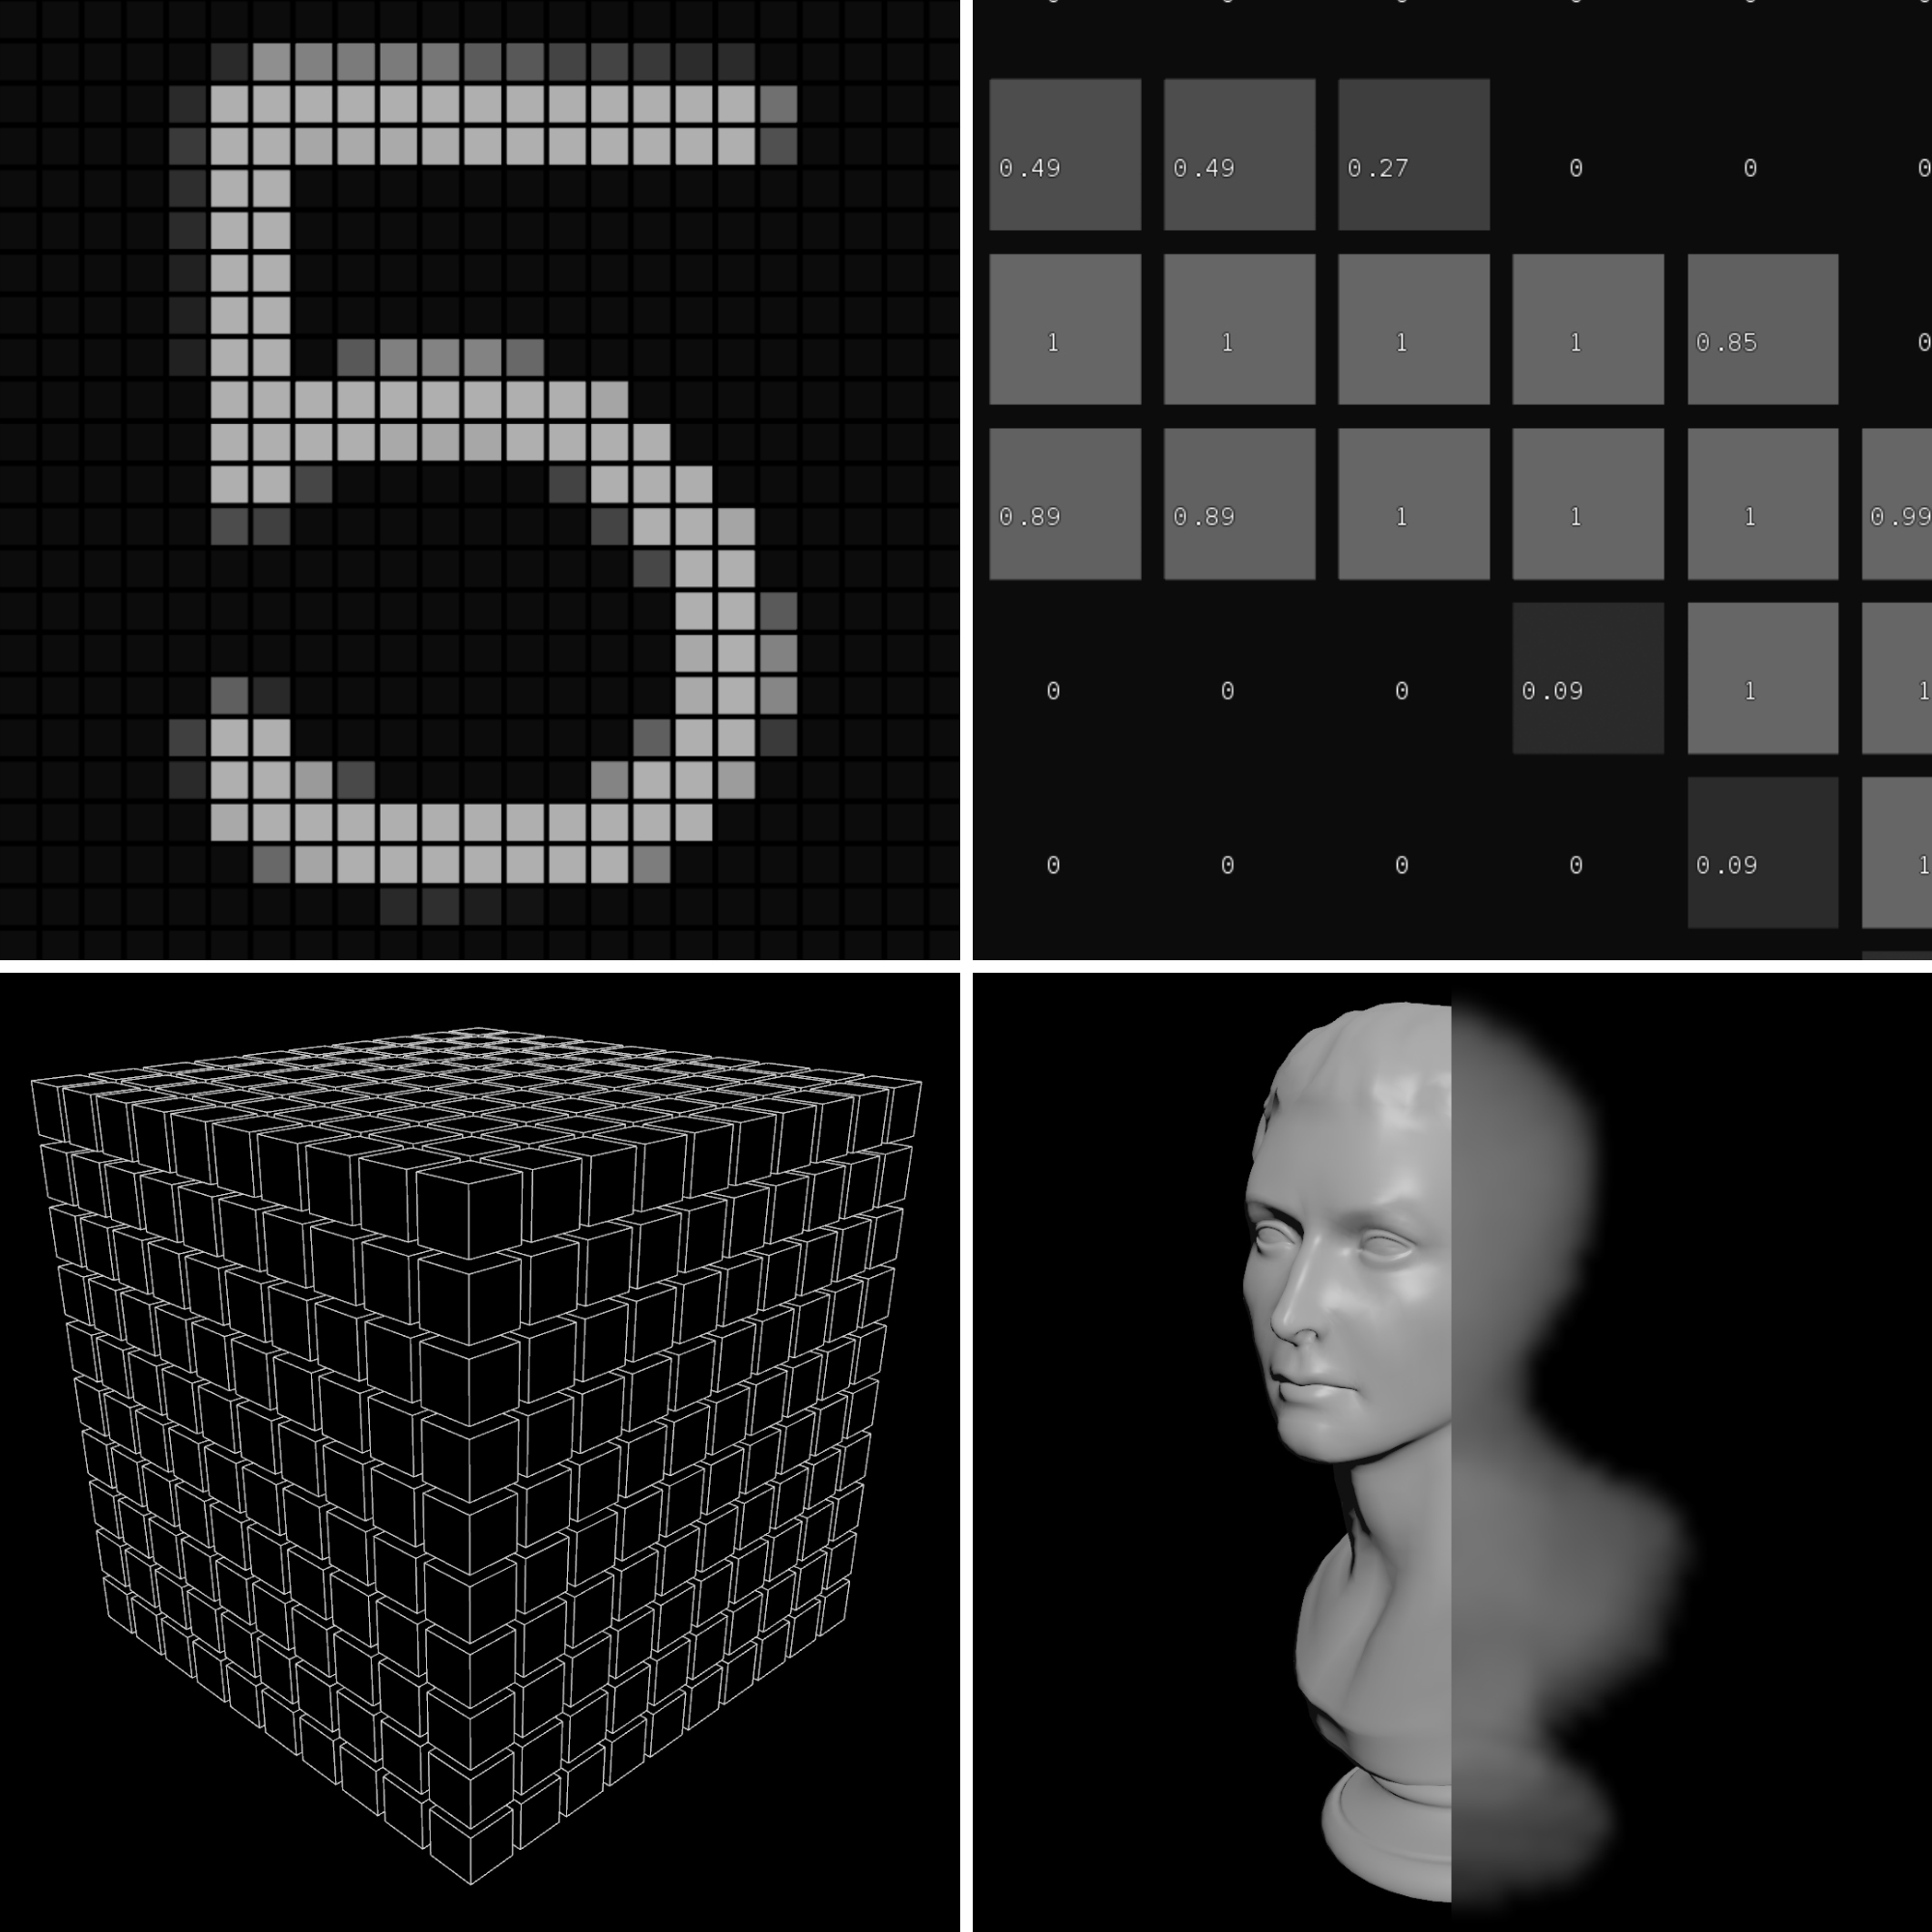
\includegraphics[width=10cm]{bilder/voxel.jpg}
    \caption{Aufbau eines Voxel Grids.}
    \source{Bild: Philipp Benner, Modell: Rico Cilliers}
    \label{voxel}
\end{figure}

Um nun Rauch oder Flammen zu simulieren, wird neben der Transparency noch einen \textit{Velocity} Wert in jedem Voxel gespeichert. Er besteht aus einem Vektor, der angibt, in welche Richtung sich der Voxel mit welcher Stärke bewegen würde, auch \textit{Advektion} genannt. Diese Werte werden während des Simulierens erzeugt und in \textit{Fields} gespeichert, wie etwa das Density und Velocity Field. Während einer Pyro-Simulation wird nun für jeden Voxel berechnet, in welche Richtung sich seine Density - basierend auf der Velocity - Frame für Frame verschiebt. Die Velocity wird dabei mit verschoben und nimmt zu oder ab, je nachdem welche physikalischen Kräfte für die Simulation eingestellt wurden. In der 3D-Simulations-Software Houdini, lassen sich komplexe Pyro-Simulationen mit weiteren Fields realisieren. Wie etwa mit dem \textit{Temperature Field}, welches die Hitzeverteilung in der Simulation speichert. Rauch oder Flammen in heißen Bereichen steigen somit schneller in der Luft auf und verteilen sich \parencite[]{understandinghowpyroworks}. Um nun eine realistisch aussehende Simulation mit vielen Details zu erhalten, muss die Anzahl an Voxel überaus hoch sein und erreicht dabei meistens den Millionenbereich.


\subsection{Water Simulations} 
Sie sind eine Mischform aus Partikel- und Pyro-Simulationen, in Houdini genannt \textit{FLIP Fluids} \parencite[]{flipsolver}. Die Partikel nehmen dabei die Rolle von Wassertropfen in der Simulation ein. Alle Informationen wie etwa die Größe, Geschwindigkeit und die Lebensspanne werden in den Partikeln gespeichert. Nur für die Berechnung der Strömung auf Grundlage der Navier-Stokes Gleichungen werden diese Informationen kurzzeitig in ein Volume übertragen \parencite[]{AlexandreJoelChorin.1967}. Dabei handelt es sich um ein Velocity Field, welches dafür sorgt, dass sich die einzelnen Partikel räumlich besser verteilen und nicht alle in dieselbe Richtung wandern \parencite[]{flipsolver}. Die Partikel lassen sich dann mit den üblichen Kräften steuern, welche auch für die einfache Partikelsimulation genutzt werden.

\section{Dateiformat OpenVDB}
Für Simulationen, die nicht auf Voxel basieren, sondern wie etwa bei Particle Simulations, lässt sich bei errechneten Frames die Position der Punkte und weitere Attribute wie Edges, Partikelgröße oder die Lebensspanne pro Partikel speichern. \\

Da Voxel hingegen Teil eines dreidimensionalen Rasters sind, müsste eine 3D-Matrix pro Field gespeichert werden, da jedes Field einen anderen Wertetyp haben kann. Die Density eines Voxels wird etwa als eindimensionale Floating Point Nummer gespeichert, das Velocity Field speichert aber einen 3D-Vektor pro Voxel, da hierbei eine Richtung angezeigt werden muss. Dabei entsteht das Problem, dass innerhalb einer Pyro-Simulation oft viele Voxel existieren, die keine wichtigen Informationen beinhalten. Zum Beispiel befindet sich am Rand einer Explosion oftmals leerer Raum, an dem keine Density oder Velocity Werte vorhanden sind. Die gespeicherte 3D-Matrix würde also aus vielen Nullen bestehen und somit unnötigen Speicherplatz verbrauchen.\\

Um diesem Problem entgegenzutreten, nutzt Houdini unter anderem das weitverbreitete Dateiformat \textit{OpenVDB} \parencite[]{openvdb}, um Voxel zu speichern \parencite[]{volumesopenvdb}. Dabei werden mithilfe der Datenstruktur eines $B^{+}$-Baumes nur Voxel zur Speicherung aktiviert, in denen auch nützliche Informationen zu finden sind. Dieses Dateiformat ermöglicht es, die Daten kompakt zu speichern und sie schnell wieder einzulesen. Beispielsweise benötigen OpenVDB Volumes 50\% weniger Speicherplatz im RAM und 13-25\% weniger Platz auf der Festplatte, als andere, für diesen Zweck optimierte Dateiformate \parencite[S. 27:18]{10.1145/2487228.2487235}.

\section{Optimierung von Simulationen}
Es existieren also eine Vielzahl an komplexen Vorgängen, die beim Simulieren eine Rolle spielen. Es gibt verschiedene Techniken, die für bestimmte Arten von Simulationen zum Einsatz kommen, welche mit teilweise gänzlich anderen Datenstrukturen arbeiten. Eine Simulation anzufertigen kann Tage dauern und sie verbraucht ebenso mehrere Terabyte Festplattenspeicher.\\

Da Visual Effects und die damit einhergehenden Simulationen in Zukunft weiterhin eine große Rolle spielen werden, steht die Forschung in diesem Bereich nicht still. Auch die steigende Leistung von Computerhardware bietet neue Möglichkeiten. Mittlerweile lassen sich Simulationen teilweise schneller und effizienter auf einer Grafikkarte anstatt dem Prozessor berechnen. Für Simulationen in geringer Auflösung ist dies sogar schon in Echtzeit möglich \parencite[S. 9]{Real-Time-incompressible}.\\

Forscher untersuchen unter anderem auch stetig, wie mit künstlicher Intelligenz Simulationen optimiert werden können. Es gelang ihnen etwa, eine künstliche Intelligenz so zu trainieren, dass sie die physikalischen Gesetze der echten Welt berücksichtigt \parencite[]{physicsinformed}. Einer anderen Gruppe ist es gelungen, Flüssigkeiten mit einem Deep Neural Network zu simulieren \parencite[]{deepfluid}. Beide Forschungsarbeiten bieten große Vorteile, da sie auf Simulationssoftware mit komplexen Algorithmen verzichten und das neuronale Netz trotzdem in der Lage ist, erstaunliche Ergebnisse zu liefern. \\
